\begin{introduction}
    \item 基本假设在全同粒子体系中遇到的困难
    \item 置换算符
    \item 对称化假设
    \item 
\end{introduction}
%12月4日任务
\section{基本假设在全同粒子体系中遇到的困难}
本章我们正式的讨论多粒子体系的一些基本性质。本节我们讨论之前的几条量子力学假设在多全同粒子体系中存在的问题。

首先我们定义全同粒子。简而言之,如果两个粒子的一切固有性质(质量、自旋、电荷)完全一样,那么这两个粒子是全同的。由这个定义我们可以知道:如果一个体系含有两个全同粒子,将两个粒子交换,体系的所有性质没有发生变化。\footnote{注意,这里的固有性质相同与否与测量无关系,在无测量的情况下我们也不能将正电子与电子看作全同粒子}

值得注意的是,全同粒子的概念与粒子是经典或是量子无关,但是经典力学中由于可以准确的确定粒子每一时刻的位移和动量,从而进一步通过跟踪不同的轨道来分辨全同粒子。

但是量子力学的全同粒子系情况就有所不同,因为此时粒子不具有确定的轨道。我们可以将服从量子力学的粒子的运动视作波包的运动,于是当粒子的波包发生重叠后,我们无法通过了解每一时刻粒子的位移与动量来确定全同粒子。

一个简单的例子就是两个粒子的碰撞问题。考虑两个全同粒子相向运动\footnote{为了方便,我们人为的对粒子标号为粒子(1)和粒子(2),标号的作用仅仅是描述方便,但不代表能够分辨它们},它们的波包在初态是分开的,随着演化的进行,波包发生了重叠,此时,与波包(1)速度成$\theta$角度上的一个探测器探测到了粒子,但是我们并不能知道这个粒子是粒子(1)还是粒子(2),因为我们并不能根据探测器的测量判断粒子碰撞是沿这哪一条路径(见图\ref{fig:identicalparticles})
\begin{figure}[H]
    \centering
    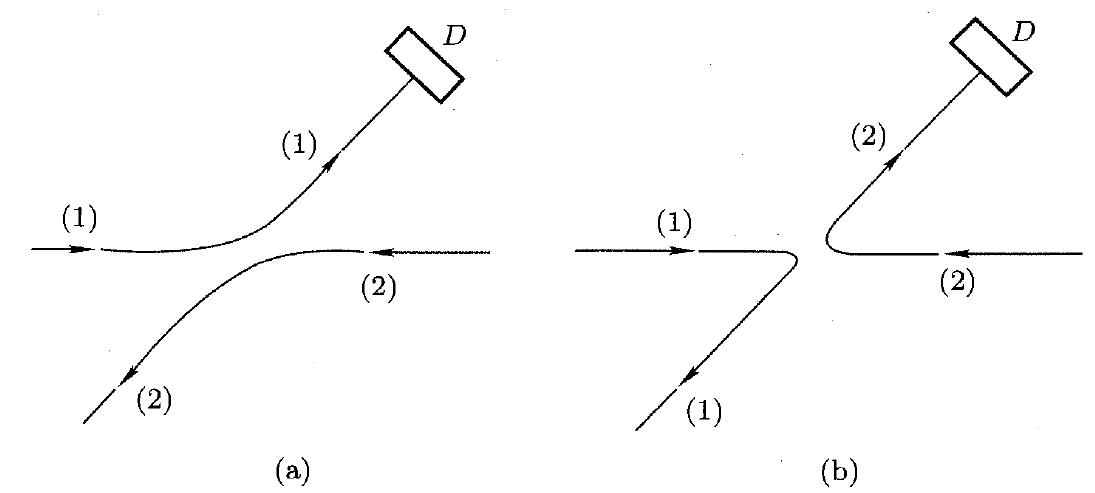
\includegraphics[width=0.6\textwidth]{figure/identicalparticles.png}
    \caption{两条可能的路径,探测器并不能分辨这两条路径对应的态}
    \label{fig:identicalparticles}
\end{figure}

上面的例子在初态的时候波包是分开的,因此初态是可以被唯一确定的,下面一个例子表明了初态也有可能不能被唯一确定,我们称这种类似的现象为交换简并。

考虑两个自旋为$\frac{1}{2}$的全同粒子,单粒子对应的自旋空间设为$\mathscr{E}_1,\mathscr{E}_2$,自旋空间上定义的自旋算符为$\hat{S_1},\hat{S_2}$。于是我们可以令$\hat{S_{1z}},\hat{S_{2z}}$的本征值为$\frac{\varepsilon_1}{2},\frac{\varepsilon_2}{2}$($\varepsilon_1,\varepsilon_2=\pm 1$)对应的共同本征态为$|\varepsilon_1,\varepsilon_2\rangle$。可以发现这个共同本征态集中存在两个态对应一个物理状态的情况,也即:
\begin{equation}
    |+,-\rangle,|-,+\rangle
\end{equation}

也就是说,该物理状态对应的右矢可以取这两个正交态张成的二维空间中的任意一个态:
\begin{equation}\label{equ11:A}
    |\psi\rangle=\alpha|+,-\rangle+\beta|-,+\rangle
\end{equation}

在上述背景下,量子力学假设应用于其上会产生问题。比如在初态为式\eqref{equ11:A}的情况下,求解为两个自旋在x轴方向本征值都为$+\frac{1}{2}\hbar$的概率,可以知道,末态应该为对应$|+\rangle_1$和$|+\rangle_2$的直积:
\begin{align}
    \begin{split}
        |\psi'\rangle=&\frac{1}{\sqrt{2}}(|\varepsilon_1=+\rangle+|\varepsilon_1\rangle)\otimes \frac{1}{\sqrt{2}}(|\varepsilon_2=+\rangle+|\varepsilon_2=-\rangle) \\
        =&\frac{1}{2}(|+,+\rangle+|+,-\rangle,|-,+\rangle,|-,-\rangle)
    \end{split}
\end{align}

于是根据量子力学假设,对应的概率为:
\begin{equation}
    P=|\langle \psi|\psi'\rangle|^2=|\frac{1}{2}(\alpha+\beta)|^2
\end{equation}

可以看到基于量子力学假设得到的概率依赖于系数$\alpha,\beta$,也即概率不确定,这是违背量子力学假设的。因此我们必须指出\eqref{equ11:A}式究竟用哪一个态而不能在二维空间中任意取,也即消除“交换简并”。

最后我们借由三全同粒子体系为例子扩展到一般N个全同粒子体系,表明全同粒子体系都会遇到交换简并的问题。对于三全同粒子体系,我们如果孤立的看待每个粒子,则每个粒子都对应一个态空间和对应的联络算符,则体系的态空间可以表示为:
\begin{equation}
    \mathscr{E}=\mathscr{E}_1\otimes\mathscr{E}_2\otimes\mathscr{E}_3
\end{equation}

设粒子(1)对应的联络算符为$\hat{B(1)}$,并且假设$\hat{B(1)}$构成$\mathscr{E}_1$的CSCO;由于三个粒子是全同粒子,因此粒子(2),(3)对应的联络算符应该为$\hat{B(2)},\hat{B(3)}$,并且本征值的谱都是相同的$\{b_i\}$,利用三个单粒子空间的基,通过张量积的形式,我们可以构造$\mathscr{E}$上的正交归一基:
\begin{equation}
    \{|1:b_i,2:b_j,3:b_p\rangle,i,j,k=1,2,\dots\}
\end{equation}

全同粒子不能让我们测量到$\mathscr{B}(1),\mathscr{B}(2),\mathscr{B}(3)$,因为粒子的编号毫无意义,但是我们可以测量物理量$\mathscr{B}$。假定测量的结果为$b_p,b_q,b_k$,则以下态是无法分辨的:
\begin{align}
    \begin{split}
        |1:b_p,2:b_q,3:b_k\rangle,&|1:b_p,2:b_k,3:b_q\rangle,|1:b_q,2:b_p,3:b_k\rangle,\\
        |1:b_q,2:b_k,3:b_p\rangle,&|1:b_k,2:b_p,3:b_q\rangle,|1:b_k,2:b_q,3:b_p\rangle
    \end{split}
\end{align}

上述交换简并导致$\hat{B}$无法分辨态空间上的这些态。我们可以很容易的推广到N个全同粒子的情况,由此我们可以看到,对于全同粒子的完全测量(与CSCO有关)不能在体系中确定唯一的态。
\section{置换算符的基本性质}
    根据上面的讨论,我们可以发现交换简并的出现实际上与标号的顺序有关,同一组数的序数排列共同构成了交换简并态。根据这个性质,我们引入了置换算符的概念来处理同一组数的序数排列问题,通过引入置换算符,我们可以简化全同粒子假设带来的推论与计算的有用工具,下面我们介绍一下基本的符号与性质。
    \subsection{两个粒子的体系}
    我们首先考虑简单情况,即自旋相同的两粒子体系。由于全同粒子带来交换简并的干扰,因此我们在本章中都人为的认为粒子都是可以分辨的,记作粒子(1)与粒子(2)。同时我们假设单粒子的自旋空间是同构的,因此对于自旋算符,$\mathscr{E}_1,\mathscr{E}_2$可以采用同一组基。于是态空间上的一组基可以表示为两个单粒子自旋空间的自旋算符对应态的张量积:
    \begin{equation}
        \mathscr{E}:|1:u_i;2:u_j\rangle
    \end{equation}
    
    定义的张量积的顺序是无关的:
    \begin{equation}
        |1:u_i;2:u_j\rangle=|2:u_i;1:u_j\rangle
    \end{equation}
    此时我们定义置换算符,它对基矢量的作用为:
    \begin{equation}
        \hat{P_{21}}|1:u_i;2:u_j\rangle=|2:u_i;1:u_j\rangle=|1:u_j;2:u_i\rangle
    \end{equation}
    
    上式说明置换算符的作用是交换两个粒子的自旋状态。置换算符具有一些良好的性质。首先,根据置换算符的定义,我们可以知道置换算符一定满足幂等性:
    \begin{equation}
        \hat{P_{21}}^2=\hat{P_{21}}
    \end{equation}
    
    同时我们也可以证明置换算符是一个厄米算符,即:
    \begin{equation}
        \hat{P_{21}}^\dagger=\hat{P_{21}}
    \end{equation}
\begin{proof}
    要想证明置换算符的厄米性,我们只需要证明算符在一组基下对应的矩阵元关系满足:
    \begin{equation}
        P_{mn}=P_{nm}^*
    \end{equation}
    
    我们考虑$\{|1:u_i;2:u_j\rangle\}$上的矩阵元:
    \begin{align}
        \begin{split}
            P_{mn}=&\langle 1:u_{i'};2:u_{j'}|\hat{P_{21}}|1:u_i;2:u_j\rangle\\
            =&\langle 1:u_{i'};2:u_{j'}||1:u_j;2:u_i\rangle\\
            =& \delta_{i'j}\delta_{ij'}\\
            P_{nm}^*=&(\langle 1:u_i;2:u_j|\hat{P_{21}}|1:u_{i'};2:u_{j'})^*\\
            =&(1:u_i;2:u_j|1:u_{j'};2:u_{i'})^*\\
            =&\delta_{i'j}\delta_{ij'}
        \end{split}
    \end{align}
    
    可以发现$\hat{P_{21}}$在$\{|1:u_i;2:u_j\rangle\}$上的矩阵元$P_{mn},P_{nm}^*$相等
\end{proof}

    根据置换算符的厄米性和幂等性,我们可以知道置换算符是幺正的:
    \begin{equation}
       \hat{P_{21}}\hat{P_{21}}^\dagger =(\hat{P_{21}})^2=\hat{I}
    \end{equation}
    
    由于置换算符是厄米的,因此它的本征值是实数,设$|\psi\rangle$是$\hat{P_{21}}$的本征态,由于幂等性,因此$\hat{P_{21}}^2$的本征值为1:
    \begin{equation}
        \hat{P_{21}}^2|\psi\rangle=|\psi\rangle
    \end{equation}
    
    所以$\hat{P_{21}}$的本征值为+1或-1,其中我们称本征值为+1的本征态是对称态,记作$|\psi_S\rangle$;本征值为-1的本征态为反对称态,记作$|\psi_A\rangle$:
    \begin{align}
        \begin{split}
            \hat{P_{21}}|\psi_S\rangle=&|\psi_S\rangle\\
             \hat{P_{21}}|\psi_A\rangle=&-|\psi_A\rangle
        \end{split}
    \end{align}
    
    在得到了对称态与反对称态的概念以后,接下来我们考虑如何通过构造投影算符构造对称态与反对称态,我们引入两个与$\hat{P_{12}}$有关的算符\footnote{在后面的内容中我们将会知道为什么算符会呈现这样的形式}:
    \begin{align}
        \begin{split}
            \hat{S}=&\frac{1}{2}(1+\hat{P_{21}})\\
            \hat{A}=&\frac{1}{2}(1-\hat{P_{21}})
        \end{split}
    \end{align}
    
    可以验证,$\hat{S},\hat{A}$同样满足幂等性,厄米性和幺正性。同时我们根据定义可以知道$\hat{S}$和$\hat{A}$是对易和互补的,即:
    \begin{align}
        \hat{S}\hat{A}=\hat{A}\hat{S}=&0\\
        \hat{S}+\hat{A}=&\hat{I}
    \end{align}
        
    上式说明$\hat{S}$和$\hat{A}$对态空间上任意态的投影作用可以构造两个互补的正交子空间\footnote{因为对于态空间上任意的态$|\psi\rangle$,都满足:
    \begin{align*}
        \hat{S}(\hat{A}|\psi\rangle)=&0\\
        \hat{A}(\hat{S}|\psi\rangle)=&0
    \end{align*}
    }
    \subsection{N个粒子的体系}
    我们可以将两个粒子的置换算符拓展到N个粒子的体系,为了简单的说明拓展定义的变动之处,我们首先考虑N=3的情况。
    
    假设三个同构的可分辨粒子的自旋空间,同时使用同一组基底$\{u_i\}$进行描述,则整个态空间上的基可以表示为:
    \begin{equation}
        \mathscr{E}:\{|1:u_i;2:u_j;3:u_k\rangle\}
    \end{equation}
    
    其对应的6个置换算符为:
    \begin{align}
        \begin{split}
            \hat{P_{123}},& \hat{P_{132}}, \hat{P_{213}}\\
             \hat{P_{231}},& \hat{P_{312}}, \hat{P_{321}}
        \end{split}
    \end{align}
    
    置换算符作用到对应的基矢量的表达式为:
    \begin{equation}
        \hat{P_{npq}}|1:u_i;2:u_j;3:u_k\rangle=|n:u_i;p:u_j;q:u_k\rangle
    \end{equation}
    
    其中$n,p,q$是1,2,3的一种序数排列。通过观察$N=3$的6个置换算符,我们可以简单验证,这6个置换算符的集合构成一个群。
    \begin{proof}
        简单验证一下六个置换算符的集合构成一个置换群。
        
        首先可以通过下表验证封闭性:
        \begin{table}[h]
            \centering
           \begin{tabular}{ |c||c|c|c|c|c|c|  }
         \hline
         \quad&$\hat{P_{123}}$& $\hat{P_{132}}$&$\hat{P_{213}}$&$\hat{P_{231}}$&$\hat{P_{312}}$&$ \hat{P_{321}}$\\
         \hline\hline
          $\hat{P_{123}}$&$\hat{P_{123}}$&$ \hat{P_{132}}$&$\hat{P_{213}}$&$\hat{P_{231}}$&$\hat{P_{312}}$&$ \hat{P_{321}}$\\
         \hline
         $\hat{P_{132}}$&$\hat{P_{132}}$&$\hat{P_{123}}$&$\hat{P_{312}}$&$\hat{P_{213}}$&$\hat{P_{321}}$&$\hat{P_{231}}$\\
         \hline
         $\hat{P_{213}}$&$\hat{P_{213}}$&$\hat{P_{231}}$&$\hat{P_{123}}$&$\hat{P_{321}}$&$\hat{P_{132}}$&$\hat{P_{312}}$\\
         \hline
         $\hat{P_{231}}$&$\hat{P_{231}}$&$\hat{P_{213}}$&$\hat{P_{321}}$&$\hat{P_{123}}$&$\hat{P_{132}}$&$\hat{P_{312}}$\\
         \hline
         $\hat{P_{312}}$&$\hat{P_{312}}$&$\hat{P_{321}}$&$\hat{P_{132}}$&$\hat{P_{231}}$&$\hat{P_{123}}$&$\hat{P_{213}}$\\
         \hline
         $\hat{P_{321}}$&$\hat{P_{321}}$&$\hat{P_{312}}$&$\hat{P_{231}}$&$\hat{P_{132}}$&$\hat{P_{213}}$&$\hat{P_{123}}$\\
         \hline
        \end{tabular}
            \caption{三个全同粒子的置换算符乘法表}
            \label{permutationgroup}
        \end{table}
        
        由上表我们可以发现,对于三全同粒子体系,任意两个置换算符$\hat{P_\alpha}$,$\hat{P_{\beta}}$,我们总能找到一个置换算符$\hat{P_\gamma}$,满足$\hat{P_\alpha}\hat{P_{\beta}}=\hat{P_{\gamma}}$。此外同样根据上表我们可以验证乘法的分配律和结合律,这个集合的单位元是$\hat{P_{123}}$,每个置换算符的逆元是它本身。
    \end{proof}
    
    类似的,我们可以拓展到N个粒子的体系,对应定义N!个置换算符,并且这N!个置换算符构成一个置换群。与两全同粒子体系类似,我们在这里引入两个重要的算符$\hat{S},\hat{A}$,其定义为:
    \begin{align}
        \begin{split}
            \hat{S}=&\frac{1}{N!}\sum_\alpha \hat{P_\alpha}\\
            \hat{A}=&\frac{1}{N!}\sum_\alpha \varepsilon_\alpha\hat{P_\alpha}
        \end{split}
    \end{align}
    
    其中当$\alpha$为偶排列时,$\varepsilon=+1$;当$\alpha$为奇排列时,$\varepsilon=-1$。可以发现在两粒子的体系中,我们定义的算符是上式的一个特例;并且在这个特例中,我们知道这两个算符是两个正交子空间的投影算符,并且定义了对称态与反对称态,类似的,在N个全同粒子体系中我们也能定义:
    \begin{align}
        \begin{split}
            \hat{P_\alpha}|\psi_S\rangle=&|\psi_S\rangle\\
            \hat{P_\alpha}|\psi_A\rangle=&\varepsilon_\alpha|\psi_A\rangle
        \end{split}
    \end{align}
    
    我们称$|\psi_S\rangle$为完全对称态,称$|\psi_A\rangle$为完全反对称态。
    \begin{remark}
    在上面的叙述中我并没有说$\hat{S},\hat{A}$将态拆成两个正交子空间,态只有对称态与放对称态,因为当$N>2$的时候,由于奇排列的出现导致这条性质不成立。比如对于$N=3$的全同粒子体系:
    \begin{equation}
        \hat{S}+\hat{A}=2(\hat{P_{123}}+\hat{P_{231}}+\hat{P_{312}})\ne \hat{I}
    \end{equation}
    \end{remark}
    
    此外,在两全同粒子体系中还证明了$\hat{S},\hat{A}$是并且满足幂等性,厄米性,对易性。那么N个全同粒子的体系定义的算符是否满足这些性质呢?首先由于$\hat{P_\alpha}$都是厄米的,因此$\hat{S},\hat{A}$也是厄米的,即:
    \begin{align}
        \begin{split}
            \hat{S}^\dagger=&\hat{S}\\
            \hat{A}^\dagger=&\hat{A}
        \end{split}
    \end{align}
    
    其次,对于某个置换算符$\hat{P_{\alpha_0}}$,我们可以有以下关系:
    \begin{align}\label{equ11:B}
        \begin{split}
            \hat{P_{\alpha_0}}\hat{S}=&\hat{S}\\
            \hat{P_{\alpha_0}}\hat{A}=&\varepsilon_{\alpha_0}\hat{A}
        \end{split}
    \end{align}
    
    由于置换算符是封闭的,因此对于给定的两个置换算符$\hat{P_{\alpha_0}},\hat{P_\alpha}$,一定存在一个置换算符$\hat{P_\beta}$满足$\hat{P_{\alpha_0}}\hat{P_\alpha}=\hat{P_\beta}$。同时,对于$\hat{A}$来说,常数$\varepsilon$也满足对应关系:$\varepsilon_\beta=\varepsilon_{\alpha_0}\varepsilon_\alpha$根据这个性质,考虑某个置换算符$\hat{P_{\alpha_0}}$对$\hat{S}$的作用,则有:
    \begin{equation}
        \hat{P_{\alpha_0}}\hat{S}=\frac{1}{N!}\sum_\alpha \hat{P_{\alpha_0}}\hat{P_\alpha}=\frac{1}{N!}\sum_\beta \hat{P_\beta}=\hat{S}
    \end{equation}
    
    同理,用同样的思路可以得到$\hat{P_{\alpha_0}}$对$\hat{S}$的作用:
    \begin{equation}
        \hat{P_{\alpha_0}}\hat{A}=\frac{1}{N!}\sum_\alpha \varepsilon_\alpha\hat{P_{\alpha_0}}\hat{P_\alpha}=\frac{1}{N!}\varepsilon_{\alpha_0}\sum_\beta \hat{P_\beta}=\varepsilon_{\alpha_0}\hat{A}
    \end{equation}
    
    如果$\hat{P_{\alpha_0}}$右乘在$\hat{S},\hat{A}$旁,证明是类似的。
    
    根据\eqref{equ11:B},我们可以推得:
    \begin{align}
        \begin{split}
            \hat{S}^2=&\hat{S}\\
            \hat{A}^2=&\hat{A}
        \end{split}
    \end{align}
    
    同时,$\hat{A}$和$\hat{S}$之间是对易的,即:
    \begin{equation}
        \hat{A}\hat{S}=\hat{S}\hat{A}=0
    \end{equation}
    
    这是因为:
    \begin{align}
        \begin{split}
            \hat{S}^2=&\frac{1}{N!}\sum_\alpha\hat{P_\alpha}\hat{S}=\frac{1}{N!}\sum_\alpha\hat{S}=\hat{S}\\
            \hat{A}^2=&\frac{1}{N!}\sum_\alpha\varepsilon_\alpha\hat{P_\alpha}\hat{A}=\frac{1}{N!}\sum_\alpha\hat{A}=\hat{A}
        \end{split}
    \end{align}
    
    上两式的最后一个等号是由于$\alpha$共有N!种排列,并且$\hat{S},\hat{A}$与$\alpha$无关。对易关系也是类似的证明:
    \begin{equation}
        \hat{A}\hat{S}=\frac{1}{N!}\sum_\alpha\varepsilon_\alpha\hat{P_\alpha}\hat{S}=\frac{1}{N!}\sum_\alpha\varepsilon_\alpha\hat{S}=\frac{\hat{S}}{N!}\sum_\alpha \varepsilon_\alpha=0
    \end{equation}
    
    其中,上式最后一个等号是因为对于数排列$\alpha$,奇排列个数等于偶排列个数。由此,我们证明了$\hat{S},\hat{A}$是态空间$\mathscr{E}$的两个正交子空间$\mathscr{E}_S,\mathscr{E}_A$的投影算符,即:
    \begin{align}
        \hat{S}\hat{P_\alpha}=\hat{P_\alpha}\hat{S}|\psi\rangle=&\hat{S}|\psi\rangle\\
        \hat{A}\hat{P_\alpha}=\hat{P_\alpha}\hat{A}|\psi\rangle=&\varepsilon_\alpha\hat{A}|\psi\rangle
    \end{align}
    在N个全同粒子体系中构造的两个投影算符$\hat{S},\hat{A}$和它们导出的一系列性质在后续说明的过程中起到非常重要的作用。
\section{对称化假设}
    \subsection{对称化假设的引入与交换简并的消除}
    为了消除交换简并带来的困难,我们引入对称化假设:
    \begin{definition}{对称化假设}{symmetry}
        对于全同粒子体系,如果交换粒子,对应的物理右矢只能是完全对称的或是完全反对称的。如果物理右矢是完全对称的,对应的粒子称为玻色子;如果物理右矢是完全反对称的,对应的粒子称为费米子。
    \end{definition}
    
    上述定义表明全同粒子的态空间不再是$\mathscr{E}$,而是其子空间,是$\mathscr{E}_S$还是$\mathscr{E}_A$取决于粒子的性质。我们知道引入对称化假设的目的在于消除交换简并,那么对称化假设是如何消除交换简并的呢?
    
    首先回顾一下前面的内容,假设$|u\rangle$是N个全同粒子体系的一个完全确定的状态,根据上面内容的讨论,我们可以知道$\hat{P_\alpha}|u\rangle$和$|u\rangle$可以描述同一个物理状态。换句话说一个物理状态位于由$\hat{P_\alpha}|u\rangle$的全体构成的态空间$\mathscr{E}$的子空间$\mathscr{E}_u$。如果$dim\mathscr{E}_u>1$,则会出现交换简并现象。而对称化假设告诉我们,描述物理状态的右矢一定位于$\mathscr{E}_S$中(如果粒子是玻色子)或者$\mathscr{E}_A$中(如果粒子是费米子)。那么问题就转换为了我们需要证明:$\mathscr{E}_u$只含有$\mathscr{E}_S/\mathscr{E}_A$的一个右矢。
    
    根据上一节的推导,我们知道投影算符满足关系:$\hat{S}=\hat{S}\hat{P_\alpha}$,$\hat{A}=\varepsilon_\alpha\hat{A}\hat{P_\alpha}$。于是对于态空间$\mathscr{E}$上任意的一个完全确定的态$|u\rangle$,我们知道:
    \begin{align}
        \begin{split}
            \hat{S}=&\hat{S}(\hat{P_\alpha}|u\rangle)\\
            \hat{A}=&\varepsilon_\alpha\hat{A}(\hat{P_\alpha}|u\rangle)
        \end{split}
    \end{align}
    
    上式说明$|u\rangle$和所有$\hat{P_\alpha}|u\rangle$在$\mathscr{E}_S$或$\mathscr{E}_A$中的投影都是共线的。也就是说,我们只需要求出$\hat{S}|u\rangle$或$\hat{A}|u\rangle$就能作为物理状态唯一的右矢了(以下简称为物理右矢)。
    \subsection{物理右矢的构造}\label{subsection:physicalket}
    根据上面的讨论,我们知道物理右矢的构造分为3步:
    \begin{itemize}
        \item 对所有粒子编号(编号仅仅为了书写的方便,而不是表明粒子之间是可分辨的),通过单粒子空间上的基构造态空间上的与某个物理状态对应的态$|u\rangle$;
        \item 根据粒子是玻色子还是费米子,将$\hat{S}$算符或者$\hat{A}$算符作用到$|u\rangle$上;
        \item 对物理右矢进行归一化;
    \end{itemize}
    
    为了生动的理解构造的过程,我们举一个简单的例子。考虑两全同粒子体系,我们令粒子(1)处于已经归一化的单粒子态$|\phi\rangle$上,令粒子(2)处于另一个已经归一化的单粒子态$|\chi\rangle$上,那么:
    \begin{equation}
        |u\rangle=|1:\phi;2:\chi\rangle
    \end{equation}
    
    如果粒子是玻色子的话,则物理右矢可以表示为:
    \begin{equation}
        \hat{S}|u\rangle=\frac{1}{2!}(\hat{P_{12}}+\hat{P_{21}})|u\rangle=\frac{1}{2}(|1:\phi;2:\chi\rangle+|1:\chi;2:\phi\rangle)
    \end{equation}
    
    如果粒子是费米子的话,则物理右矢可以表示为:
    \begin{equation}
        \hat{A}|u\rangle=\frac{1}{2!}(\varepsilon_{12}\hat{P_{12}}+\varepsilon_{21}\hat{P_{21}})|u\rangle=\frac{1}{2}(|1:\phi;2:\chi\rangle-|1:\chi;2:\phi\rangle)
    \end{equation}
    
    最后考虑归一化,如果$|\phi\rangle$和$|\chi\rangle$是正交的,那么归一化因子很容易求出:只要将上述两式前的系数换成$\frac{1}{\sqrt{2}}$即可。
    \begin{remark}
    考虑一种特殊情况:$|\phi\rangle=|\chi\rangle$,此时观察费米子的物理右矢,你会发现$\hat{A}|u\rangle=\frac{1}{2}(|1:\phi;2:\phi\rangle-|1:\phi;2:\phi\rangle)=0$,也就是说当费米子处于两个相同的单粒子态的时候,$\mathscr{E}_A$中没有一个非平凡的右矢可以代表这个物理状态,这种情况下是违背对称化假设的,我们称其为Pauli不相容原理。这个原理在后续的讨论中有重要意义。
    \end{remark}
    
    对于N=3的情况,我们可以类似的令$|u\rangle$的形式为:
    \begin{equation}
        |u\rangle=|1:\phi;2:\chi;3:\varphi\rangle
    \end{equation}
    
    则对于玻色子的情况,物理右矢可以表示为:
    \begin{align}
         \begin{split}
             \hat{S}|u\rangle=&\frac{1}{3!}(|1:\phi;2:\chi;3:\varphi\rangle+|1:\phi;3:\chi;2:\varphi\rangle+|2:\phi;1:\chi;3:\varphi\rangle+\\
             &|2:\phi;3:\chi;1:\varphi\rangle+|3:\phi;1:\chi;2:\varphi\rangle+|3:\phi;2:\chi;1:\varphi\rangle)
         \end{split}
    \end{align}
       
     对于费米子来说,物理右矢可以表示为:
     \begin{align}
         \begin{split}
             \hat{S}|u\rangle=&\frac{1}{3!}(|1:\phi;2:\chi;3:\varphi\rangle-|1:\phi;3:\chi;2:\varphi\rangle-|2:\phi;1:\chi;3:\varphi\rangle+\\
             &|2:\phi;3:\chi;1:\varphi\rangle+|3:\phi;1:\chi;2:\varphi\rangle-|3:\phi;2:\chi;1:\varphi\rangle)
         \end{split}
    \end{align}
    
    可以发现,上式的定义正好符合行列式的定义\footnote{因为行列式其中一种定义正好也是与数的奇排列偶排列有关},于是我们可以写成一个更紧凑的行列式形式,即Slater行列式:
    \begin{equation}
        \hat{A}|u\rangle=\frac{1}{3!}\begin{vmatrix}
            |1:\phi\rangle&|1:\chi\rangle&|1:\varphi\rangle\\
            |2:\phi\rangle&|2:\chi\rangle&|2:\varphi\rangle\\
            |3:\phi\rangle&|3:\chi\rangle&|3:\varphi\rangle
        \end{vmatrix}
    \end{equation}
    
    如果有两个单粒子态相同,则有行列式中有两列相同,因此行列式等于0,因此Pauli不相容原理在N=3也是成立的。如果$|\phi\rangle,|\chi\rangle,|\varphi\rangle$是正交的,那么归一化只要将$\frac{1}{3!}$换成$\frac{1}{\sqrt{3!}}$即可。
    
    类似的结论可以推广到N个全同粒子的体系,即我们可以用单粒子态去构成玻色子的物理右矢;用Slater行列式构成费米子的物理右矢。同时由于行列式的特殊性导致Pauli不相容原理仍然成立,这一点造成了费米子与玻色子的区别。
    \begin{remark}
        Pauli不相容原理会导致玻色子和费米子的性质有很大的不同。其中,玻色子在低温出现的一种现象被称为玻色-爱因斯坦凝聚,其本质就在于在低温的时候,玻色子能够“一窝蜂”地挤到最低能级中去,而费米子却要受到Pauli不相容原理的限制。一个著名的例子就是He-3具有的超流动性,就是因为He-3是玻色子。
    \end{remark}
    \subsection{构成物理右矢基的构造}
    本节我们讨论N个全同粒子的体系如何构造物理右矢的一组基:首先我们选择单粒子态空间上的一组基$\{|u_i\rangle\}$构成态空间$\mathscr{E}$上的一组基:
    \begin{equation}
        \mathscr{E}:\{|1:u_i;2:u_j;\dots;N:u_p\rangle\}
    \end{equation}
    
    根据对称化假设,物理右矢一定位于$\mathscr{E}_S$或$\mathscr{E}_A$上,因此我们考虑$\hat{S}/\hat{A}$作用于基$\{|1:u_i;2:u_j;\dots;N:u_p\rangle\}$上,得到张成空间$\mathscr{E}_S$或$\mathscr{E}_A$的矢量集合。
    \begin{remark}
    比如我们考虑一个在$\mathscr{E}_S$空间上的态$|\varphi\rangle$,由于$\mathscr{E}_S$一定是$\mathscr{E}$的一个子空间,则$|\varphi\rangle$一定可以可以用$\mathscr{E}$上的基$\{|1:u_i;2:u_j;\dots;N:u_p\rangle\}$线性表示:
    \begin{equation}
        |\varphi\rangle=\sum_{i,j,\dots,p}a_{i,j,\dots,p}|1:u_i;2:u_j;\dots;N:u_p\rangle
    \end{equation}
    
    根据定义:$|\varphi\rangle\in\mathscr{E}_S$,因此一定有关系:
    \begin{equation}
        \hat{S}|\varphi\rangle=|\varphi\rangle
    \end{equation}
    
    联立两式可得:
    \begin{equation}
         |\varphi\rangle=\sum_{i,j,\dots,p}a_{i,j,\dots,p}(\hat{S}|1:u_i;2:u_j;\dots;N:u_p\rangle)
    \end{equation}
    
    可以发现:$\hat{S}|1:u_i;2:u_j;\dots;N:u_p\rangle$就是张成空间$\mathscr{E}_S$的矢量集合。
    \end{remark}
    
    但是这样运算存在一个问题,即$\hat{S}|1:u_i;2:u_j;\dots;N:u_p\rangle$并不是线性无关的!(比如$\hat{S}\hat{P_\alpha}|1:u_i;2:u_j;\dots;N:u_p\rangle$就与$\hat{S}|1:u_i;2:u_j;\dots;N:u_p\rangle$对应同一个物理状态)。为了解决这个问题,我们引入占有数的概念\footnote{这个概念的提出非常自然,我的理解是,全同粒子的问题本质上就是相同小球的排列组合问题,我们需要时刻考虑到单纯排列带来的重复}:
    \begin{definition}{占有数}{occupynumber}
        对于态$|1,u_i;2,u_j;\dots;N,u_p\rangle$,单粒子态$|u_k\rangle$的占有数$n_k$等于$|u_k\rangle$在$\{|u_i\rangle,|u_j\rangle,\dots,|u_p\rangle\}$中出现的次数。
    \end{definition}
    
    如果对于各单粒子态的占有数分别是相等的,则态可以通过置换算符的作用进行转换,并且这些转换的态对应同一个物理右矢,记作$|n_1,n_2,\dots,n_k\rangle$,称为粒子数表象。这个概念将会在后续的二次量子化中继续深入讨论。

    \section{与其它量子力学假设的相容性}
    本节主要想论证在对称化假设的框架下,其它量子力学假设也能与之相容,其中主要包含两点:
    \begin{itemize}
        \item 只使用$\mathscr{E}_S$/$\mathscr{E}_A$中的物理右矢去描述测量过程;
        \item $|\psi(t)\rangle$经过演化后不会超出$\mathscr{E}_S$/$\mathscr{E}_A$
    \end{itemize}
    
    换句话说,我们希望其它量子力学假设在$\mathscr{E}_S$/$\mathscr{E}_A$空间上成立。
    
        \subsection{与测量与算符假设的相容}
        我们假设测量前的态是$|\psi(t)\rangle$;显然,根据对称化假设,$|\psi(t)\rangle$一定属于$\mathscr{E}_S$或$\mathscr{E}_A$。经过测量物理量$\mathscr{A}$以后,态变为了物理右矢$|u\rangle$,其中$|u\rangle$可以通过\ref{subsection:physicalket}节中的方法构造。如此,初态和末态都在$\mathscr{E}_S$/$\mathscr{E}_A$中,那么所有量子力学的结果就取决于标量积$\langle \psi|u\rangle$和矩阵元$\langle\psi|\hat{A}|u\rangle$了,我们先考虑标量积$\langle \psi|u\rangle$。
        
                \begin{remark}
        全同粒子的测量与非全同粒子的测量有什么不同呢?我们在第二章讲述概率幅与测量的关系的时候曾经见过一个连续测量的例子:如果我们对中间态进行测量,那么我们必须对概率幅进行求和,这样就产生了干涉效应;而如果我们确定了一个具体的中间态的话,那么我们只能根据经典粒子的情况对概率分别进行求和,干涉效应消失。在这里是一样的想法,由于全同粒子的特点,其根据对称性与反对称性构造的物理右矢$|u\rangle$相当于中间态,当对全同粒子进行测量的时候,我们应该对概率幅相加,此时会产生由交换导致的干涉效应;而当粒子非全同的时候,相当于我们确认了全同粒子全排列中的一种,此时测量,干涉效应消失。
        
        为了方便理解,这里举一个两个全同粒子测量的例子。假设两个全同粒子在测量前处于两个相互正交的单粒子态$|\chi\rangle,|\varphi\rangle$,则根据对称化假设,对应的物理右矢应该满足:
        \begin{equation}
            |\varphi,\chi\rangle=\frac{1}{\sqrt{2}}(1+\varepsilon\hat{P_{21}})|1:\varphi;2:\chi\rangle
        \end{equation}
        
        其中:
        \begin{equation}
            \varepsilon=\left\{
            \begin{array}{cc}
                +1 & \text{粒子是玻色子} \\
                -1 & \text{粒子是费米子}
            \end{array}
            \right.
        \end{equation}
        
        当体系处于$|\varphi,\chi\rangle$态时,对整个体系进行物理量$\mathscr{B}$的测量,对应的测量算符满足下列本征方程:
        \begin{equation}
            \hat{B}|u_i\rangle=b_i|u_i\rangle
        \end{equation}
        
        我们要考虑的问题是求得特定结果($b_m,b_n$)的概率。此时,末态根据对称化假设可以得到:
        \begin{equation}
            |u_m,u_n\rangle=\frac{1}{\sqrt{2}}(1+\varepsilon\hat{P_{21}})|1:u_m;2:u_n\rangle
        \end{equation}
        
        因此,概率幅可以表示为:
        \begin{equation}
            \langle u_m,u_n|\varphi,\chi\rangle=\frac{1}{2}\langle 1:u_m;2:u_n|(1+\varepsilon\hat{P_{21}}^\dagger)(1+\varepsilon\hat{P_{21}})|1:\varphi;2:\chi\rangle
        \end{equation}
        
        由于:
        \begin{align}
            \begin{split}
                \frac{1}{2}(1+\varepsilon\hat{P_{21}}^\dagger)(1+\varepsilon\hat{P_{21}})=&\frac{1}{2}\big(1+\varepsilon(\hat{P_{21}}^\dagger+\hat{P_{21}})+\varepsilon^2\hat{P_{21}}^2\big)\\
                =&\frac{1}{2}\big(1+\varepsilon(\hat{P_{21}}^\dagger+\hat{P_{21}})+1\big)\\
                =&1+\varepsilon \hat{P_{21}}
            \end{split}
        \end{align}
        
        代入概率幅公式可以得到:
        \begin{align}
            \begin{split}
                 \langle u_m,u_n|\varphi,\chi\rangle=&\frac{1}{2}\langle 1:u_m;2:u_n|(1+\varepsilon\hat{P_{21}})|1:\varphi;2:\chi\rangle\\
                 =&\langle 1:u_m;2:u_n|1:\varphi;2:\chi\rangle+\varepsilon\langle 1:u_m;2,u_n|1:\chi;2:\varphi\rangle\\
                 =&\langle 1:u_m|1:\varphi\rangle\langle 2:u_n|2:\chi\rangle+\varepsilon\langle 1:u_m|1:\chi\rangle\langle2:u_n|2:\varphi\rangle\\
                 =& \langle u_m|\varphi\rangle\langle u_n|\chi\rangle+\varepsilon\langle u_m|\chi\rangle\langle u_n|\varphi\rangle
            \end{split}
        \end{align}
        
        上式可以理解为初态到末态的两条路径的干涉(形象的表示如图\eqref{fig:identical_interfere}),于是目标的概率为:
        \begin{equation}
            P(b_m;b_n)=| \langle u_m,u_n|\varphi,\chi\rangle|^2
        \end{equation}
        
        \begin{figure}[H]
            \centering
            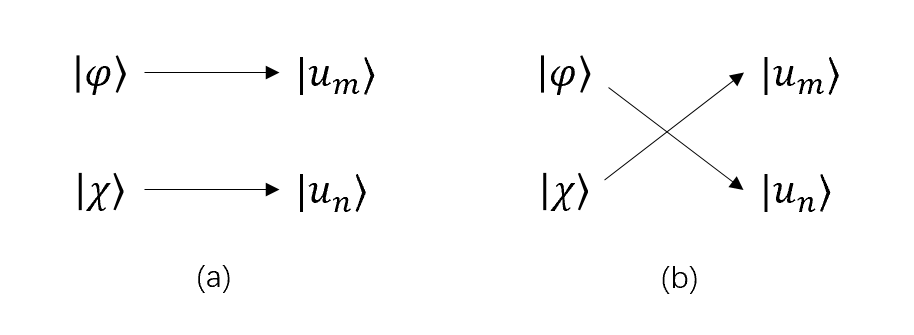
\includegraphics[width=0.9\textwidth]{figure/identical_interfere.png}
            \caption{两全同粒子体系的直接项(a)与交换项(b)的示意图}
            \label{fig:identical_interfere}
        \end{figure}
        
        通常我们称概率幅公式的第一项为直接项,第二项为交换项。当体系是全同粒子态的时候,直接项的概率幅与交换项的概率幅会产生干涉。其中,玻色子以"+"干涉,费米子以"-"干涉。
        \end{remark}
        
        显然,根据上面的描述,标量积可以通过$\mathscr{E}_S$/$\mathscr{E}_A$中的两个矢量进行描述,不同的地方在于:如果$\hat{A}$是一个完全的测量(就是构成$\mathscr{E}_S/\mathscr{E}_A$上的ESCO,比如测量全体粒子的位移$r$和自旋分量$S_x$),则$|u\rangle$一定是唯一的;如果$\hat{A}$是一个不完全的测量(就是不构成$\mathscr{E}_S/\mathscr{E}_A$上的ESCO),则物理右矢$|u\rangle$有若干个(并且是相互正交的)。
        \begin{remark}
        比如我们考虑态空间$\mathscr{E}$上的一个态$|1:u_i;2:u_j;\dots;N:u_p\rangle$,完全测量就是完全确定了全同粒子状态的集合$\{|u_i\rangle,|u_j\rangle,\dots,|u_p\rangle\}$,则根据对称化假设的讨论,符合条件的物理右矢是唯一的;不完全测量指的就是不能完全获得全同粒子的状态(比如仅仅测量了1个粒子的位移和自旋或是只测了所有粒子的自旋),这样我们知道满足条件的物理状态不止一个,自然物理右矢$|u\rangle$也不止一个。但是由于本征态的性质,不同本征态对应的右矢是正交的,因此不同的$|u\rangle$也是正交的。
        \end{remark}
       
        接下来我们讨论算符假设的相容性。什么算符能够表示全同粒子系的物理状态呢?我们抓住全同粒子系本身的特点,即交换粒子并不会改变体系的物理状态,也就是说,如果对于物理状态$|u\rangle$,用$\hat{G}$测量$|u\rangle$以后,交换粒子并不会改变测量后的物理状态$\hat{G}|\psi\rangle$。由于置换算符有关系:
        \begin{equation}
            \hat{P_\alpha}|\psi\rangle=\varepsilon_\alpha|\psi\rangle
        \end{equation}
        
        那么上述论述可以表示为:
        \begin{equation}
            \hat{P_\alpha}\hat{G}|\psi\rangle=\hat{G}\hat{P_\alpha}|\psi\rangle=\varepsilon_\alpha\hat{G}|\psi\rangle
        \end{equation}
        
        由此我们可以知道,描述物理状态的算符$\hat{G}$与置换算符之间满足关系:
        \begin{equation}\label{equ11:communitive}
            [\hat{G},\hat{P_\alpha}]=0
        \end{equation}
        
        上式一方面表明$\hat{G}$在$\mathscr{E}_S/\mathscr{E}_A$下不变;同时也表明算符$\hat{G}$对所有粒子具有交换对称性。
        
        \subsection{与Schrodinger方程的相容}
        本节考虑状态演化的相容性,考虑在$\mathscr{E}_S/\mathscr{E}_A$下的一个含时物理右矢$|\psi(t)\rangle$,我们知道Schrodinger方程:
        \begin{equation}
            i\hbar\frac{d|\psi(t)\rangle}{dt}=\hat{H}|\psi(t)\rangle
        \end{equation}
        
        由于$d|\psi(t)\rangle=|\psi(t+dt)\rangle-|\psi(t)\rangle$,因此上式可以化简为:
        \begin{equation}
            |\psi(t+dt)\rangle=\big(1+\frac{dt}{i\hbar}\hat{H}\big)|\psi(t)\rangle
        \end{equation}
        
        我们将$\hat{P_\alpha}$作用于上式,结合\eqref{equ11:communitive}式,我们可以得到:
        \begin{equation}
            \hat{P_\alpha}|\psi(t+dt)\rangle=\hat{P_\alpha}\big(1+\frac{dt}{i\hbar}\hat{H}\big)|\psi(t)\rangle=\big(1+\frac{dt}{i\hbar}\hat{H}\big)(\hat{P_\alpha}|\psi(t)\rangle)
        \end{equation}
        
        该式表明$\hat{P_\alpha}|\psi(t)\rangle$经过演化得到$\hat{P_\alpha}|\psi(t+dt)\rangle$。进一步,如果$|\psi(t)\rangle$是$\hat{P_\alpha}$的本征态,那么$|\psi(t+dt)\rangle$也是$\hat{P_\alpha}$的本征态并且本征值相同,因此粒子是费米子还是玻色子并不随着状态的演化而改变。换句话说Schrodinger方程并不会使$|\psi(t)\rangle$的演化超出$\mathscr{E}_S/\mathscr{E}_A$。